%\newpage
%============================================================================================================================


\chapter{Построение графов через реализацию графа на плоскости}

\chapter{Реализация графа в Coq}

\section{Представление графов в Coq}
Реализации графов из статьи де Грея приведены в файле {\tt myGraphs.v}~\ref{lst:myGraphs}
Представление графа было взято из книги Softwarefoundations \cite{VFA}.
Для представления графа используются модули {\tt FSets} и {\tt FMaps}, которые предоставляют интерфейсы множества и отображения. Эти модули принимают различные типы ключей, в данном случае мы будем использовать тип позитивных чисел {\tt positive} из модуля {\tt PositiveOrderedTypeBits}.

\begin{verbatim}
Module E := PositiveOrderedTypeBits.
Module S <: FSetInterface.S := PositiveSet.
Module M <: FMapInterface.S := PositiveMap.
\end{verbatim} 

Вершина {\tt node} -- это элемент типа {\tt positive}, {\tt nodemap} -- это отображение из вершин, а граф {\tt graph} -- это отображение из типа вершина в тип множество вершин. Тип {\tt positive} был выбран из-за того, что в нем оператор сравнения определен так, чтобы поиск по ключу типа {\tt positive} в множестве и отображении был более эффективным.

\begin{verbatim}
Definition node := E.t.
Definition nodeset := S.t.
Definition nodemap: Type -> Type := M.t.
Definition graph := nodemap nodeset.
\end{verbatim}

Для работы с графами были определены функции добавления ребра в существующий граф и построения графа из списка ребер.

\begin{verbatim}
Definition add_edge (e: (E.t*E.t)) (g: graph) : graph :=
 M.add (fst e) (S.add (snd e) (adj g (fst e))) 
  (M.add (snd e) (S.add (fst e) (adj g (snd e))) g).
\end{verbatim}

В данной функции ребро представляется парой вершин.
В данной работе реализуются неориентированные графы без петель.

\begin{verbatim}
Definition mk_graph (el: list (E.t*E.t)) :=
  fold_right add_edge (M.empty _) el.
\end{verbatim}

В терминах определенных выше функций построение графа {\tt K3} выглядит следующим образом:
\begin{verbatim}
Definition K3 := 
    mk_graph [ (1, 2) ; (2, 3); (1, 3)].
\end{verbatim}

Далее для работы с графом можно использовать функцию вывода множества вершин и функцию вывода множества ребер.
\begin{verbatim}
Compute (S.elements (Mdomain K3)).
(* 
    = [2; 1; 3]
        : list S.elt.
*)
\end{verbatim}

\begin{verbatim}
Function gr_show (g : graph) : list (node * node) :=
  S.fold 
    (fun n l => (map (fun y => (n, y)) (S.elements (adj g n))) ++ l) 
    (Mdomain g) nil.
\end{verbatim}

\begin{verbatim}
Compute gr_show K3.
(*
= [(3, 2); (3, 1); (1, 2); (1, 3); (2, 1); (2, 3)]
    : list (node * node)
*)
\end{verbatim}

Граф H построен на основе графа {\tt K3} с помощью нескольких вспомогательных функций.


Рекурсивная функция {\tt l\_rng} находит минимум и максимум в списке, функция {\tt gr\_rng} находит в графе минимальный и максимальный номера вершин.

\begin{verbatim}
Fixpoint l_rng' (l : list node) (cur_min: node) (cur_max: node) : 
    node * node :=
  match l with
  | nil => (cur_min, cur_max)
  | x :: xs  => 
        let cur_min := if x <? cur_min then x else cur_min in
        let cur_max := if cur_max <? x then x else cur_max in
        l_rng' (xs) (cur_min) (cur_max)
  end.

Function l_rng (l : list node) :=
  match l with
    | nil => (1%positive, 2%positive)
    | x::xs =>  l_rng' l  x x
  end.

Function gr_rng (g : graph) : node * node :=
  l_rng (S.elements (Mdomain g)).
\end{verbatim}


  
\begin{verbatim}
Definition mk_cmn_edge (g1 g2 : graph) (a b n m : node) : graph :=
(* Make graphs disjoint. *)
  let g2' := rename_all (fun x => x + snd (gr_rng g1)) g2 in
(* New names for the edge's vertices. *)
  let n' := n + snd (gr_rng g1) in
  let m' := m + snd (gr_rng g1) in
 (* Delete adge from second graph *)
  let g2' := delete_edge g2' n' m' in
  let g_result :=  S.fold 
                    (fun m g' => M.add m (adj g2' m) g') 
                    (Mdomain g2') g1 in
  let g_result := rename_node n' a g_result in 
  rename_node m' b g_result.
\end{verbatim}

\begin{verbatim}
Definition L: graph :=
  let KK := mk_art K K A A in
  let KK := add_edge (B, B+snd(gr_rng K)) KK in
  rename_in_order KK.
\end{verbatim} 

\section{Доказательства корректности операций над графами}

\chapter{Доказательство свойств раскраски малых графов в Coq}
Назовем две раскраски $f$, $f'$ графа $G$ $существенно одинаковыми$, если существуют изоморфизм графа $g$ и перестановка цветов $ \omega $ такие, что
$f(v) = \omega ( f'( g(v) ) )$ . Также назовем две раскраски $существенно различными$, если они не являются существенно одинаковыми.

{\it Граф H} -- это граф $$H := (\{1, 2, 3, 4, 5, 6, 7 \},$$
    $$ \{(1, 2), (1, 3), (1, 4), (1, 5), (1, 6), (1, 7), $$
    $$ (2, 3), (3, 4), (4, 5), (5, 6), (6, 7), (7, 2)\}) $$
    

\begin{figure}[ht] 
  \center
  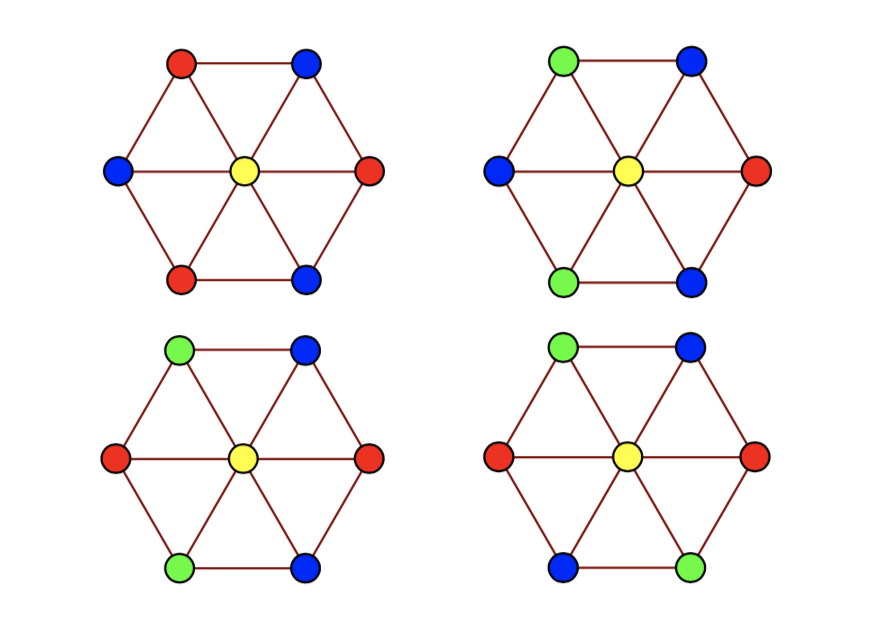
\includegraphics [width=0.8\linewidth] {Colorings_of_H}
  \caption{Существенно различные способы раскрасить граф H в не более чем 4 цвета} 
  \label{img:Colorings_of_H}
\end{figure}

В статье \cite{deGrey} утверждается что существует только 4 существенно различные раскраски графа {\tt H} в не более чем в 4 цвета. Это утверждение обосновывается перебором вариантов наличия или отсутствия монохроматических троек.

\section{Про {\tt Ltac}, {\tt pattern matching} и {\tt goal matching} }
В данной главе активно используется язык {\tt Ltac} и инструмент {\tt goal matching}, представляемый этим языком.

\section{Типы возможных правильных раскрасок графа {\tt T} в не более чем 4 цвета}

Назовем {\it тройкой} любой граф, изоморфный графу {\it T} на четырех вершинах $$T := (\{1, 2, 3, 4\} , \{(1, 2), (1, 3), (1, 4) \} )$$.

{\it Утверждение}: Существует только три существенно различные раскраски графа $G$, если граф $G$ изомрфен $T$.

В системе Coq это раскраски можно описать следующим образом:

\begin{verbatim}
(* Monochromatic *)
Definition type1_triple (el: list node) (c: Coloring) :=
  let center := nth 0 el 1 in
  let v1 := nth 1 el 1 in
  let v2 := nth 2 el 1 in
  let v3 := nth 3 el 1 in
  let c1 := c center in
  let c2 := c v1 in
  ~ (c1 = c2) /\ same_color c v1 v2 /\ same_color c v2 v3.

(* 2 and 1 *)
Definition type2_triple (el: list node) (c: Coloring) :=
  let center := nth 0 el 1 in
  let v1 := nth 1 el 1 in
  let v2 := nth 2 el 1 in
  let v3 := nth 3 el 1 in

  let c1 := c center in
  let c2 := c v1 in
  let c3 := c v2 in 
  let c4 := c v3 in
  ~ (c1 = c2) /\ ~ (c1 = c3) /\ ~ (c1 = c4) /\
    ( (c2 = c3 /\ ~ c2 = c4) \/ (c2 = c4 /\ ~ c2 = c3) \/ 
        (c3 = c4 /\ ~ c3 = c2) ).

(* All 3 different *)
Definition type3_triple (el: list node) (c: Coloring) :=
  let center := nth 0 el 1 in
  let v1 := nth 1 el 1 in
  let v2 := nth 2 el 1 in
  let v3 := nth 3 el 1 in

  let c1 := c center in
  let c2 := c v1 in
  let c3 := c v2 in 
  let c4 := c v3 in
  ~ (c1 = c2) /\ ~ (c1 = c3) /\ ~ (c1 = c4) /\
    (~ c2 = c3) /\ (~ c2 = c4) /\ (~ c3 = c4).
\end{verbatim}

Каждая функция имеет тип {\tt Prop}, принимает на вход список вершин и раскраску, при этом первый элемент в списке -- номер вершины, соединенной со всеми остальными. Формула {\tt type1\_triple} кодирует то, что все вершины, кроме первой одинакового цвета, при этом этот цвет отличен от цвета первой вершины. Формула {\tt type2\_triple} кодирует то, что цвет первой вершины отличен от цвета остальных вершин, а среди остальных есть две одинакового цвета, который отличен от цвета оставшейся вершины. Формула {\tt type3\_triple} кодирует случай, когда все 4 вершины имеют различный цвет.

Теорема {\tt my\_Triple\_Coloring} утверждает, что любая правильная раскраска графа {\tt T} является раскраской одного из этих типов. Ее доказательство включает в себя перебор всех возможных раскрасок, однако благодаря использованию языка {\tt Ltac} и {\tt goal matching} можно переиспользовать куски доказательства в ситуациях, отличающихся только перестановкой цветов или изоморфизма графа.

Полный код доказательства приведен в файле {\tt my\_Triple\_Coloring.v}~\ref{lst:my_Triple_Coloring}. Тактика {\tt contr} доказывает {\tt my\_Triple\_Coloring} от противного и применяется в случаях, когда раскраска не является правильной, т.~е. существует пара смежных ребер одного цвета. Тактика {\tt type1\_tac} применяется, когда полученная раскраска является раскраской первого типа, тактики {\tt type1\_tac\_left}, {\tt type1\_tac\_middle} {\tt type1\_tac\_right} -- раскраской второго типа (различны раскраски на различные случаи, какая пара вершин является парой одного цвета) и тактика {\tt type3\_tac} применяется для доказательства того, что раскраска является раскраской третьего типа.

Таким образом, для любой раскраски графа T существует тактика, с помощью которой можно доказать утверждение о том, что если раскраска правильная, то она является раскраской одной из трех типов. Теперь все эти тактики можно объединить в одну тактику {'\tt level4}, которая с помощью {\tt goal matching} может определить, какую именно тактику из указанных использовать. Теперь можно создать тактики {\tt level3} и {\tt level2}, которые также с помощью {\tt goal matching} определяют, необходимо ли доказывать утверждение от противного или вызывать тактику следующего уровня.

Итак, благодаря {\tt goal matching} доказательство утверждения при различных контестах может быть доказано одной и той же тактикой, что позволяет использовать конвейер и записать доказательство теоремы очень кратко

\begin{verbatim}
Lemma coloring_triple_T:
  forall c: Coloring, is_good_coloring c T ->
  type1_triple [1; 2; 3; 4] c \/ type2_triple [1; 2; 3; 4] c \/
  type3_triple [1; 2; 3; 4] c.
Proof.
  intros. unfold is_good_coloring in H. unfold is_coloring in H. 
  destruct H. remember H as H'. clear HeqH'. 
  specialize (H' 1). inversion H';
    remember H as H''; clear HeqH''; specialize (H'' 2); 
    inversion H''; remember H0 as H0'; clear HeqH0';
      level2 H H0' H0 H2 H3 c.
Qed.
\end{verbatim}

\section{Типы возможных правильных раскрасок графа {\tt H} в не более чем 4 цвета}

Теперь, когда доказано утверждение про правильные раскраски {\it троек}, можно перейти к раскраскам графа {\tt H}.

{\it Граф H} -- это граф $$H := (\{1, 2, 3, 4, 5, 6, 7 \},$$
    $$ \{(1, 2), (1, 3), (1, 4), (1, 5), (1, 6), (1, 7), $$
    $$ (2, 3), (3, 4), (4, 5), (5, 6), (6, 7), (7, 2)\}) $$

\chapter{Алгоритм раскраски графа из статьи де Грея}

\section{Работа алгоритма на Python}
\section{Реализация алгоритма в Coq}
\label{chapt1}





\chapter{Заключение}

\section{Выводы}
В данной работы были разработаны методы построения и графов, а также верифицирована корректность операций над ними. Формализованы и верифицированы утверждения о том, что есть не более 4 существенно различных способа раскрасить граф {\tt H} в не более, чем 4 цвета, а также алгоритм перебора возможных раскрасок графа, использующий алгоритм возврата.

\section{Планы будущей работы}
Разработанные методы можно использовать для верификации других статей про раскраски графов, например, статьи Marijn~J.H.~Heule, <<Computing Small Unit-Distance Graphs with Chromatic Number 5>>~\cite{Huele}.

Также разработанную технику можно использовать в автоматизации поиска графов меньших размеров, которые не красятся в 4 цвета, а также поиска графов, которые не красятся в 5 цветов.

\chapter{Приложение}

Листинг~\ref{lst:myGraphs} подгружается из внешнего файла. 

\begingroup
    \lstinputlisting[caption={Листинг myGraphs.v},label={lst:myGraphs}]{listings/myGraphs.v}
\endgroup
 
\begingroup
    \lstinputlisting[caption={Листинг myGraphs\_Properties.v},label={lst:myGraphs}]{listings/myGraphs_Properties.v}
\endgroup

\begingroup
    \lstinputlisting[caption={Листинг my\_New\_Coloring.v},label={lst:my_New_Coloring}]{listings/my_New_Coloring.v}
\endgroup


\begingroup
    \lstinputlisting[caption={Листинг my\_Triple\_Coloring.v},label={lst:my_Triple_Coloring}]{listings/my_Triple_Coloring.v}
\endgroup


\begingroup
    \lstinputlisting[caption={Листинг my\_H\_coloring.v},label={lst:my_H_coloring}]{listings/my_H_coloring.v}
\endgroup
 
  
\label{chapt1}
